\chapter{Background}
\label{chap:background}

The purpose of this chapter is to briefly recall some preliminaries related to our work, including concepts from model-driven engineering, as well as formal and stochastic modeling. As our work attempts to aid the calculation of stochastic metrics based on engineering models, we also describe the stochastic analysis tasks that we are aiming to support.

\Cref{chap:rgspn} builds on generalized stochastic Petri nets, which are described in \vref{ssec:background:gspn}, in order to define a formalism suitable for analysis model fragments. \Cref{chap:transform} uses incremental query execution of graph patterns, which are described in \vref{ssec:background:patterns}, to instantiate the analysis model fragments according to a changing domain model. Lastly, \cref{chap:apply} discusses the application of the transformation toolchain to aid proposing and solving stochastic analysis task from \vref{ssec:background:analysis} in design-space exploration for the calculation of stochastic metrics on engineering models.

Furthermore, \vref{ex:background:running} introduces the \emph{dining philosophers} problem, which is used as a running example throughout this thesis.

\section{Modeling and metamodeling}

In model-driven engineering \emph{models} provide abstractions of reality, including the structure and the behavior of systems we wish to analyze or design~\citep{Giese06multiparadigm}. The models are described in some \emph{formalism} or \emph{modeling language}.

The syntax of modeling languages is traditionally partitioned into \emph{abstract} and \emph{concrete syntax}. Concrete syntax provides a textual or graphical representation of the modeling language. Abstract syntax is endowed with meaning by mapping into a \emph{semantic domain}, which is another modeling language on a lower abstraction level.

\subsection{Metamodels and instance models}

Metamodels explicitly describe the abstract syntax of modeling languages. We will adopt the formal description of metamodels as first-order logical structures from the work of \citet{Varro17generation} and extend them to support primitive-valued attributes. Metamodels are regarded as first-order signatures:

\begin{dfn}
  A \emph{metamodel} is a first-order two-sorted logical signature
  \begin{equation}
    \Sigma = \{\lit C_1, \lit C_2, \ldots, \lit C_n; \lit R_1, \lit R_2, \ldots, \lit R_m; \lit A_1, \lit A_2, \ldots, A_k\} \text,
  \end{equation}
  where
  \begin{compactitem}
  \item \OBJsort\ and \PRIMsort\ are the sorts of objects and primitives, respectively;
  \item \(\lit C_1, \lit C_2, \ldots, \lit C_{\mathrlap{n}\phantom{m}} \ofkind \OBJsort\) are unary relation symbols called \emph{classes};
  \item \(\lit R_1, \lit R_2, \ldots, \lit R_m \ofkind \OBJsort \times \OBJsort\) are binary relation symbols called \emph{references} (or \emph{edges});
  \item \(\lit A_1, \lit A_2, \ldots, \lit A_{\mathrlap{k}\phantom{m}} \ofkind \OBJsort \times \PRIMsort\) are binary relation symbols called \emph{attributes}.
  \end{compactitem}
\end{dfn}

Instances of metamodels are regarded as first-order structures:

\begin{dfn}
  An \emph{instance model} \(M = \ltup \Obj, \Prim, \II \rtup\) of the metamodel \(\Sigma\) is a first-order two-sorted structure, where
  \begin{compactitem}
  \item \(\Obj = \{o_1, o_2, \ldots, o_N\}\) is a finite set of \emph{objects} (or \emph{individuals});
  \item \(\Prim\) is a set of possible primitive values of attributes, for example, \(\Prim \subseteq \RR \cup \BB\), where \(\RR\) is the set of real numbers and \(\BB = \{\lit{true}, \lit{false}\}\);
  \item \(\II\colon \Sigma \to \Obj \cup (\Obj \times \Obj) \cup (\Obj \times \Prim)\) is the \emph{interpretation function}, such that
    \begin{compactitem}
    \item \(\II(\lit C_i) = \lit C_i^M \subseteq \Obj\) for all classes \(\lit C_i \in \Sigma\);
    \item \(\II(\lit R_i) = \lit R_i^M \subseteq \Obj \times \Obj\) for all references \(\lit R_i \in \Sigma\);
    \item \(\II(\lit A_i) = \lit A_i^M \subseteq \Obj \times \Prim\) for all attributes \(\lit A_i \in \Sigma\).
    \end{compactitem}
  \end{compactitem}
\end{dfn}

Existing metamodeling technologies, such as the Ecore metamodeling language from the Eclipse Modeling Framework (\textabbr{EMF})~\citep{Steinberg09emf} often allow the designers of modeling languages to impose additional constraints on instances models. Some possible restrictions are listed below: 
\begin{itemize*}
\item \emph{Class inheritance} may specify that instances of a class must be instances of another.
\item \emph{Abstract classes} and \emph{interfaces} can have no direct instances.
\item \emph{Type constraints} on references and attributes restrict the class of the object originating the reference or attribute and the class of the object at the end of the reference, as well as the type of the primitive attribute value.
\item \emph{Multiplicity constraints} place lower or upper bounds on the number of references or attributes from an object.
\item Objects may be organized into a \emph{containment hierarchy,} in which an object is either a \emph{containment root,} or is connected to its \emph{container} in the hierarchy with exactly one \emph{containment} reference. The containment hierarchy forms a forest of containment roots, which is traversed when the object graph is serialized.
\item \emph{Opposite constants} require some references to always go in a direction opposite to another, i.e.~\(\lit{R}(o_i, o_j)\) should hold if and only if we have \(\lit{R}^{\textrm{op}}(o_j, o_i)\).
\end{itemize*}

Further \emph{well-formedness constraints} may be specified with \emph{constraint languages,} such as the object constraint language~(\textabbr{OCL})~\citep{OMG14ocl} or with graph patterns~\citep{Bergmann11validation}.

\begin{figure}%
  \begin{minipage}[t]{0.3333\textwidth}
    \centering
    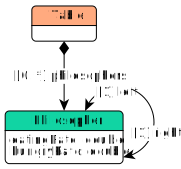
\includegraphics[scale=0.9]{figures/phil_cd}
    \caption{\protect\RaggedRight Class diagram for the dining philosophers metamodel.}
    \label{fig:background:metamodel}
  \end{minipage}%
  \begin{minipage}[t]{0.3333\textwidth}
    \centering
    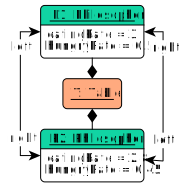
\includegraphics[scale=0.9]{figures/phil_instance}
    \caption{\protect\RaggedRight Instance model with two philosophers.}
    \label{fig:background:instance}
  \end{minipage}%
  \begin{minipage}[t]{0.3333\textwidth}
    \centering
    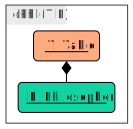
\includegraphics[scale=0.9]{figures/q_phil_pattern}
    \caption{\protect\RaggedRight Example graph query matching a philosopher at a table.}
    \label{fig:background:pattern}
  \end{minipage}%
\end{figure}

\begin{runningExample}\label{ex:background:running}
  We now introduce the \emph{dining philosophers} domain, which will be used as a running example throughout this thesis. A number of philosophers sit around a circular table, such that each philosopher has someone on her left and also on her right. Each philosopher has a single fork. The forks are placed between philosophers so that adjacent philosophers must share a fork. A philosopher can only think if she is not hungry and can only eat if she is holding both forks from her left and right.

  Philosophers have a \emph{hungry rate}, which determines how often they get hungry and a \emph{eating rate} which determines how fast they eat. We are interested in evaluating seating plans (arrangements) of philosophers to determine the total amount of philosophical knowledge produced, i.e.~the time the philosophers spent thinking. By swapping philosophers around the table we can avoid seating two gluttonous philosophers or two slow eaters next to each other; thus we can minimize the contentions for forks that prevent philosophers from satiating their hunger before they can resume thinking.

  \Vref{fig:background:metamodel} shows a class diagram for the metamodel of the dining philosophers problem. It contains two classes, \lit{Table} and \lit{Philosopher}, three relations, \lit{philosophers}, \lit{left}, \lit{right}, as well as two attributes, \lit{eat\-ing\-Rate} and \lit{hung\-ry\-Rate}.

  Type constraints require that \lit{philosophers} connect \lit{Table} objects to \lit{Philosopher} objects. It is also a containment reference, which makes \lit{Table} the root of the containment hierarchy. Moreover, the multiplicity bound \lit{[0..*]} allows any number of philosophers around the table, even zero.

  The relations \lit{left} and \lit{right} connect \lit{Philosopher} instances. The relation \lit{right} is the opposite of \lit{left}; therefore the philosopher on the left of someone sees that person on her right and vice verse. Due to the multiplicity bounds \lit{[1]} each philosopher must have a single left and right neighbor.

  \Vref{fig:background:instance} shows an instance model with a single \lit{Table} \lit{T} and two \lit{Philosopher} instances \lit{P1} and \lit{P2}. Because there are only two philosophers around the table, both philosophers see the other on their left, as well as on their right.
\end{runningExample}

\subsection{Graph patterns}
\label{ssec:background:patterns}

State-of-the-art modeling toolchains often rely of model queries to retrieve fragments of interest from model, to specify model to model and model to text transformations, as well as to validate well-formedness constraints on models~\citep{Bergmann11validation,Ujhelyi15incquery}.

Formally, again following \citet{Varro17generation}, we define a graph query \(\phi(x_1, x_2, \ldots, x_n)\) with \(n\) free variables as a first-order logic formula over the metamodel signature \(\Sigma\). The formula may contain atomic propositions of the form \(\lit C_i(x_j)\), \(\lit R_i(x_j, x_\ell)\) and \(\lit A_i(x_j, x_\ell)\), where \(\lit C_i, \lit R_i, \lit A_i \in \Sigma\) are classes, references and attributes, respectively. Furthermore, logical connectives \(\neg, \land, \lor, \Rightarrow\) and quantifiers \(\exists, \forall\) may also appear in formulas.

Model query engines often allow transitive closure computation \(\phi^+\), which makes the query language strictly more expressive than first-order logic. If \(\phi\) is a formula with two free variables, its transitive closure \(\phi^+(x_i, x_j)\) holds if and only if there are some objects \(x_i = y_1, y_2, \ldots, y_k = x_j\) (\(k \ge 1\)) such that we have \(\phi(y_1, y_2) \land \phi(y_2, y_3) \land \cdots \land \phi(y_{k - 1}, y_k)\)~\citep{Bergmann12incscc}.

For detailed semantics of first-order graph patterns extended with transitive closure we refer to the works of \citet{Semerath17rewriting} and \citet{Varro17generation}.

The tuple \(\ltup q_1, q_2, \ldots, q_n \rtup \in (\Obj \cup \Prim)^n\) is a \emph{match} of \(\phi(x_1, x_2, \ldots, x_n)\) in the instance model \(M\) if \(\phi\) holds with the \emph{match arguments} \(\ltup q_1, q_2, \ldots, q_n \rtup\), i.e.~\(M \vDash \phi(q_1, q_2, \ldots, q_n)\). We will occasionally write the name of the graph pattern before the tuple to emphasize that it is a tuple of match arguments, e.g.~\(\phi\ltup q_1, q_2, \ldots, q_n\rtup\).

The \emph{match set} of the pattern \(\phi\) in the instance model \(M\) contains all of its matches. It is a set, i.e.~it contains each tuple at most once, regardless how many valid bindings are possible for the quantified variables inside the pattern.

An \emph{incremental} (or \emph{live}) query engine, such as \textabbr{VIATRA} Query~\citep{Ujhelyi15incquery} maintains the match sets of graph queries by subscribing to \emph{change notifications} from the instance model. The changes are propagated to the match sets, and clients may get notifications about matches appearing and disappearing as the instance model is being modified. The Rete algorithm~\citep{Forgy82rete} is often employed for change propagation.

\begin{runningExample}
  Consider the instance model from \vref{fig:background:instance} along with the graph pattern
  \begin{equation}
    \lit{qPhil}(x_1, x_2) = \lit{Table}(x_1) \land \lit{Philosopher}(x_2) \land \lit{philosophers}(x_1, x_2) 
  \end{equation}
  depicted in \vref{fig:background:pattern}, which matches philosophers sitting at a table. Its match set contains two tuples, \(\lit{qPhil}\ltup \lit{T}, \lit{P1}\rtup\) and \(\lit{qPhil}\ltup \lit{T}, \lit{P2}\rtup\), which correspond to the two philosophers in the model.
\end{runningExample}

\section{Formal models for stochastic analysis}

In this section we recall some of the basic formalisms involved in our work. Petri nets are introduced firstly, which serve as the basis in our framework to express stochastic models. Then we move to the background in stochastic modeling and analysis methods. Portions of this section were adapted from previous work by \citet[Chapter~2]{Klenik15configurable}.

Throughout this section and the rest of this work \(\NN\), \(\NNpos\), \(\RR\), \(\RRpos\) will refer to the sets of natural numbers including zero \(\NN = \{0, 1, 2, \ldots\}\), the set of positive natural numbers \(\NNpos = \NN \setminus \{0\}\), the set of real numbers and the set of positive real numbers, respectively.

\subsection{Petri nets}
\label{ssec:background:petri-nets}

Petri nets are a widely used graphical and mathematical modeling tool for systems which are concurrent, asynchronous, distributed, parallel or nondeterministic~\citep{Murata89petri}.

\begin{dfn}
  A \emph{Petri net with inhibitor arcs and priorities} is a 7-tuple
  \begin{equation}
    \textit{PN} = \ltup P, T, m_0, \pi, {\inarc}, {\outarc}, {\inharc} \rtup \text,
  \end{equation}
  where the sets \(P\) and \(T\) are disjoint and
  \begin{compactitem}
  \item \(P\) is a finite set of \emph{places};
  \item \(T\) is a finite set of \emph{transitions};
  \item \(m_0 \colon P \to \NN\) is the \emph{initial marking function};
  \item \(\pi \colon T \to \NN\) is the \emph{transition priority function};
  \item \({\outarc}, {\inarc}, {\inharc} \subseteq P \times \NNpos \times T\) are the relations of \emph{output, input} and \emph{inhibitor arcs}, respectively, which are free of parallel arcs, i.e.~\(\ltup p, n_1, t \rtup, \ltup p, n_2, t \rtup \in {\outarc}\) implies \(n_1 = n_2\) and this property holds also for \(\inarc\) and \(\inharc\).
  \end{compactitem}
\end{dfn}

We will write \(p \overset{n}{\outarc} t\), \(p \overset{n}{\inarc} t\) and \(p \overset{n}{\inharc} t\) for \(\ltup p, n, t \rtup \in {\outarc}\), \(\ltup p, n, t \rtup \in {\inarc}\) and \(\ltup p, n, t \rtup \in {\inharc}\), respectively. The arc \emph{inscriptions} are omitted in the case \(n = 1\).

Petri nets are graphically represented as edge weighted directed bipartite graphs. Places are drawn as circles, while transitions are drawn as bars or rectangles. The arc inscriptions are shown as edge weights.

A \emph{marking} \(m: P \to \NN\) assigns a number of \emph{tokens} to each place.
The transition \(t\) is \emph{enabled} in the marking \(m\) if \(m(p) \ge n\) for all \(p \overset{n}{\outarc} t\) and \(m(p) < n\) for all \(p \overset{n}{\inharc} t\).

An enabled transition is \emph{fireable}, written as \(\tranenabled{m}{t}\), if no enabled transition has higher priority, i.e.~\(\pi(t') \le \pi(t)\) for all enabled transitions \(t'\).

A fireable transition \(t\) can be \emph{fired} to yield a marking \(m'\), written as \(m \tranto{t} m'\), where \(m'(p) = m(p) - n_{\textrm{in}}+ n_{\textrm{out}}\) if \(p \xrightarrow{n_{\textrm{in}}} t\) and \(p \xleftarrow{n_{\textrm{out}}} t\). If only an input or output arc is present between \(t\) and \(p\), the token count of \(p\) is only decreased or increased, respectively. Places not connected to \(t\) by an arc have their token count unchanged.

A marking \(m'\) is \emph{reachable} from \(m\), written as \(m \reachto m'\), if there is a sequence of markings and transitions such that \(m = m_1 \tranto{t_1} m_2 \tranto{t_2} \cdots \tranto{t_{k - 1}} m_k = m'\). The \emph{reachable state space} \(\RS\) of a Petri net is the set of markings reachable from its initial marking,
\begin{equation}
  \RS = \{m\colon P \to \NN \mid m_0 \reachto m \} \text.
\end{equation}

The Petri net is \emph{bounded} if there is an upper bound \(K \in \NN\) such that \(m(p) \le K\) for all \(p \in P\) and \(m \in \RS\). The reachable state space \(RS\) is finite if and only if the net is bounded.

The state space of a bounded Petri net can be determined efficiently by the \emph{saturation} algorithm~\citep{Ciardo01saturation,Ciardo12tenyears}. Extensions have been proposed for the  algorithm to handle transition priorities effectively~\citep{Miner06saturation,Marussy17priorities}.

The arc inscriptions of a Petri net may depend on the current marking by replacing the positive integers \(\NNpos\) with a set of algebraic expressions \(\Expr_P\) over the token counts of places. In the marking dependent setting \({\outarc}, {\inarc}, {\inharc} \subseteq P \times \Expr_P \times T\) and the inscription expressions are evaluated according to the marking \(m\) when firing transitions \(m \tranto{t} m'\). Such \emph{Petri nets with marking-dependent arcs} can simplify formal modeling \citep{Ciardo93decomposition}; however, they may preclude the use of some analysis techniques.

\begin{figure}
  \centering
  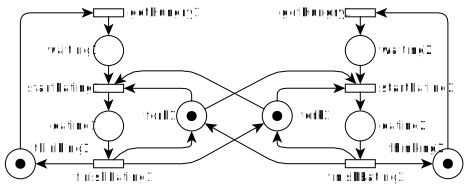
\includegraphics[scale=0.9]{figures/pn_example}
  \caption{Example Petri net with two deadlock-free dining philosophers.}
  \label{fig:background:pn-example}
\end{figure}

\begin{runningExample}\label{ex:background:pn}
  \Vref{fig:background:pn-example} shows an example Petri net modeling the dining philosophers problem with two philosophers. The philosophers \(i = 1, 2\) are modeled by the places \lit{thinking}\(i\), \lit{waiting}\(i\) and \lit{eating}\(i\). In the initial marking both philosophers are \lit{thinking}. Upon firing \lit{getHungry}\(i\) a philosopher may get hungry and starts \lit{waiting} for forks to eat with. If both \lit{fork1} and \lit{fork2} is available, she may then \lit{startEating}\(i\) by picking up both forks. The forks are picked up as a single atomic action. This avoids a possible case for deadlock when both philosophers pick up single forks but are unable to get the other fork and start eating. Therefore this model is the deadlock-free version of the dining philosophers problem. Upon finishing eating, the philosophers put their forks down by firing \lit{finishEating}\(i\) and returning to the \lit{thinking} state.
\end{runningExample}

\subsection{Continuous-time Markov chains}
\label{ssec:background:ctmc}

Continuous-time Markov chains (\textAbbr{CTMC}s) are mathematical tools for describing the behavior of systems in continuous time where the stochastic behavior of the system only depends on its current state~\citepeg{Reibman89transient}. This assumption is reasonable in a wide class of modeling tasks; hence \textAbbr{CTMC}s are commonly used in the reliability and performability prediction of critical systems.

\begin{dfn}
  A \emph{continuous-time Markov chain} (\textabbr{CTMC})
  \(X = \{ X(t) \in S \mid t \ge 0 \}\) over the finite state
  space $S = \{0, 1, \ldots, n - 1\}$ is a continuous-time random
  process with the \emph{Markovian} or memoryless property:
  \begin{multline}\allowdisplaybreaks[0]
    \Pr(X(t_k) = x_k \mid X(t_{k - 1}) = x_{k - 1}, X(t_{k -
      2}) = x_{k - 2}, \ldots, X(t_{0}) = x_{0}) \\
    = \Pr(X(t_k) = x_k \mid X(t_{k - 1}) = x_{k - 1}) \text,
  \end{multline}
  where $t_0 \le t_1 \le \cdots \le t_k$ and $X(t_k)$ is a random variable denoting the state of the \textabbr{CTMC} at time $t_k$. A \textabbr{CTMC} is said to be
  \emph{time-homogenous} if it also satisfies
  \begin{equation}
    \Pr(X(t_k) = x_k \mid X(t_{k - 1}) = x_{k - 1}) = \Pr(X(t_k - t_{k -
      1}) = x_k \mid X(0) = x_{k - 1}) \text,
  \end{equation}
  i.e.~it is invariant under time shifting. In this work we will restrict our attention to time-homogenous \textAbbr{CTMC}s over finite state spaces.
\end{dfn}

The \emph{state probabilities} at time $t$ form a finite-dimensional vector \(\vec{\uppi}(t) \in \RR^n\), where \(\pi(t)[x] = \Pr(X(t) = x)\). Following the convention from \textabbr{CTMC} literature, all vectors considered will be row vectors, i.e.~\(n\) element vectors are equivalent to matrices with a single row and \(n\) columns. Moreover, the \(i\)th element of the vector \(\vec{v}\) will be written as \(v[i]\), where indexing is zero-based (\(i = 0, 1, \ldots, n - 1\)).

The vectors \(\vec{\uppi}(t)\) satisfy the differential equation
\begin{equation}
  \label{eq:background:ctmc-diffeq}
  \frac{\dd \vec{\uppi}(t)}{\dd t} = \vec{\uppi}(t) \, Q
\end{equation}
for some square matrix $Q$. The matrix $Q$ is called the \emph{infinitesimal generator matrix} of the \textabbr{CTMC} and satisfies \(Q \vec{1}^T = \vec{0}^T\), where \(\vec{1}\) and \(\vec{0}\) are \(n\)-element vectors of ones and zeroes.

The diagonal elements \(q[x, x] < 0\) of \(Q\) describe the holding times of the \textabbr{CTMC}. If \(X(t) = x\), the \emph{holding time} \(h_x = \inf \{ h > 0 \mid X(t) = x, X(t + h) \ne x \}\) spent in state \(x\) is exponentially distributed with rate \(\lambda_x = -q[x, x]\). If \(q[x, x] = 0\) then no transitions are possible from the state $x$ and it is said to be \emph{absorbing}.

The off-diagonal elements \(q[x, y] \ge 0\) of \(Q\) describe state transitions of the \textabbr{CTMC}. The \textabbr{CTMC} while being in state \(X(t) = x\) will jump to state~\(y\) at the next state transition with probability \(-q[x, y] / q[x, x]\). Equivalently, there is an expontentially distributed countdown in the state \(x\) for each \(y\) that satisfies \(q[x, y] > 0\) with \emph{transition rate} $\lambda_{xy} = q[x, y]$. The first countdown to finish will trigger a state change to the corresponding state \(y\). Therefore the \textabbr{CTMC} is a transition system with exponentially distributed timed transitions.

\begin{figure}%
  \begin{minipage}{.5\textwidth}
    \centering
    \begin{tikzpicture}
      \matrix [column sep=1.5cm, every node/.style={inner
        sep=0pt,minimum size=.85cm, draw,circle}] {
        \node (s0) {\(0\)}; & \node (s1) {\(1\)}; & \node (s2) {\(2\)}; \\
      };
      \draw [every edge/.append style={-Latex,bend left}, every node/.append style={above}]
      (s0) edge node {\(\lambda_1\)} (s1)
      (s1) edge node {\(\lambda_2\)} (s2) (s2) edge node {\(\mu_2\)} (s1)
      (s1) edge node {\(\mu_1\)} (s0) (s2) edge [bend left=45] node {\(\mu_3\)} (s0);
    \end{tikzpicture}
  \end{minipage}%
  \begin{minipage}{.5\textwidth}
    \centering
    \(\begin{blockarray}{rccc}
      & 0 & 1 & 2 \\
      \begin{block}{r(ccc)}
        0 & -\lambda_1 & \lambda_1 & 0 \\
        Q = 1 & \mu_1 & -\lambda_2 - \mu_1 & \lambda_2 \\
        2 & \mu_3 & \mu_2 & -\mu_2 - \mu_3 \\
      \end{block}
    \end{blockarray}\)
  \end{minipage}
  \caption{Example \textabbr{CTMC} with 3 states and its generator matrix.}
  \label{fig:background:ctmc-repair}
\end{figure}

\begin{example}
  \Vref{fig:background:ctmc-repair} shows a \textabbr{CTMC} with 3 states. The transitions from the state \(0\) to \(1\) and from \(1\) to \(2\) are associated with exponentially distributed countdowns with rates \(\lambda_1\) and \(\lambda_2\) respectively, while transitions in the reverse direction have rates \(\mu_1\) and \(\mu_2\). The transition form state \(2\) to \(0\) is also possible with rate $\mu_3$.
  
  The rows \paren{corresponding to source states} and columns \paren{destination states} of the infinitesimal generator matrix \(Q\) are labeled with the state numbers. The diagonal element \(q[1, 1]\) is \(-\lambda_2 - \mu_1\), hence the holding time in state \(1\) is exponentially distributed with rate \(\lambda_2 + \mu_1\). The transition from state \(1\) to \(0\) is taken with probability \(-q[1, 0] / q[1, 1] = \mu_1 / (\lambda_2 + \mu_1)\), while the transition to \(2\) is taken with probability \(\lambda_2 / (\lambda_2 + \mu_1)\).
\end{example}

\subsubsection{Steady-state probabilities}

A state \(y\) is \emph{reachable} from the state \(x\), written as \(x \reachto y\), if there exists a sequence of states \(x = z_1, z_2, z_3, \ldots, z_{k - 1}, z_k = y\), such that \(q[z_i, z_{i + 1}] > 0\) for all \(i = 1, 2, \ldots, k - 1\). If \(x \reachto y\) for all pairs of states \(x, y \in S\), the Markov chain is \emph{irreducible}.

The \emph{steady-state probability distribution} \(\vec{\uppi} = \lim_{t \to \infty} \vec{\uppi}(t)\) exists and is independent from the \emph{initial distribution} \(\vec{\uppi}(0) = \vec{\uppi}_0\) if and only if the \textabbr{CTMC} is irreducible. The steady-state distribution satisfies the system of linear equations
\begin{equation}
  \label{eq:background:ctmc-steadystate}
  \frac{\dd \vec{\uppi}}{\dd t} = \vec{\uppi} \, Q = \vec{0},
  \quad \vec{\uppi} \vec{1}^\T = 1 \text.
\end{equation}

The matrix \(Q\) is sparse and is often amenable to decomposed storage~\citep{Buchholz99hierarchical}.
However, solving the system of linear equations~\cref{eq:background:ctmc-steadystate} requires iterative linear equation solver algorithms, which can have varying convergence and running time characteristics~\citep{Buchholz99structured,Marussy16configurable,Buccholz17compact}.

Selection of numerical solver backends and their parameters in the context of design-space exploration toolchains are discussed in \vref{ssec:apply:integration-solver}.

\subsubsection{Parametric models}

The infinitesimal generator matrix of a \emph{parametric \textabbr{CTMC}} depends on a vector of \emph{parameters} \(\vec{\uptheta} \in A \subseteq \RR^k\), where \(A\) is the \emph{feasible region} of parameter values. The parameters represent unknown or uncertain attributes of the system under study, while the feasible region describes realizable or plausible parameter values. \emph{Parameter optimization} refers to the selection of feasible parameter values \(\vec{\uptheta} \in A\) such that some \emph{goal function} is maximized.

Analysis methods for parametric Markov chains include sensitivity analysis~\citep{Blake88sensitivity}, parametric steady-state solution~\citep{Hahn11parametric,Voros17pdn} and parameter synthesis~\citep{Quatmann16mdp}. Some analysis methods only allow specific kinds of parameter-dependence in the generator matrix elements \(\vec{\uptheta} \mapsto q(\vec{\uptheta})[x, y]\), such as \(C^1\) differentiable expressions~\citep{Blake88sensitivity} or rational functions~\citep{Hahn11parametric}.

\subsubsection{Markov reward models}

Continuous-time Markov chains may be employed in the estimation of performance measures of models by defining \emph{rewards} that associate \emph{reward rates} with the states of a \textabbr{CTMC}. The reward rate random variable $R(t)$ can describe performance measures defined at a single point of time, such as resource utilization or the probability of failure, while the \emph{accumulated reward} random variable $Y(t)$ may correspond to performance measures associated with intervals of time, such as the total downtime.

\begin{dfn}
  A \emph{continuous-time Markov reward process} over a finite state space \(S = \{0, 1, \ldots, n - 1\}\) is a pair \(\ltup X, \vec{r} \rtup\), where \(X\) is a \textabbr{CTMC} over \(S\) and \(\vec{r} \in \RR^n\) is a \emph{reward rate vector}. The reward rate stochastic process \(R = \{ R(t) = r[X(t)] \mid t \ge 0 \}\) describes the momentary \emph{reward rate} associated with the active state of the \textabbr{CTMC}.

  The \emph{accumulated reward} until time \(t\) is defined as the time integral of \(R\),
  \begin{equation}
    Y = \biggl\{ Y(t) = \int_{0}^t R(\tau) \,\dd \tau \biggm\vert t \ge 0 \biggr\}\text.
  \end{equation}
\end{dfn}

\begin{example}
  Let \(c_0\), \(c_1\) and \(c_2\) denote operating costs per unit time associated with the states of the \textabbr{CTMC} \(X\) in \vref{fig:background:ctmc-repair}. Consider the Markov reward process \(\ltup X, \vec{r} \rtup\) with the reward rate vector
  \begin{equation}
    \vec{r} = \begin{pmatrix} c_0 & c_1 & c_2 \end{pmatrix} \text.
  \end{equation}
  The random variable \(R(t)\) describes the momentary operating cost, while \(Y(t)\) is the total operating expenditure until time \(t\). The steady-state expectation \(\lim_{t \to \infty} \Ex R(t)\) is the average maintenance cost per unit time of the long-running system.
\end{example}

In parameter-dependent reward models not only does the infinitesimal generator matrix \(Q\colon A \to \RR^{n \times n}\) depend on the parameter vector \(\vec{\uptheta} \in A\) but also can the reward rate vector \(\vec{r}\colon A \to \RR^n\) be parameter-dependent.

\subsection{Stochastic analysis tasks}
\label{ssec:background:analysis}

Various analysis tasks concerning \textAbbr{CTMC}s and Markov reward models are performed to calculate stochastic metrics or determine whether the system satisfies a reliability or performability requirement. We will refer to such problems as \emph{queries} concerning a stochastic model. Below we attempt to give a short summary of the most basic analyses and computational methods.

\newpara \textbf{Steady-state analysis} refers to the calculation of the steady-state expectation \(\Ex R(\infty) = \lim_{t \to \infty} \Ex R(t)\) to characterize the values of reliability or performability metrics during long-term system operation. Because the steady state expectation is calculated according to the formula \(\Ex R(\infty) = \vec{\uppi} \, \vec{r}^T\), where \(\vec{\uppi}\) is the steady-state probability vector form \vref{eq:background:ctmc-steadystate}, this form of analysis is tantamount to the solution of \cref{eq:background:ctmc-steadystate}.

\newpara \textbf{Transient and accumulated analysis} is concerned with the transient behavior of the modeled system when it is started from an initial probability distribution \(\vec{\uppi}_0\). An initial value problem with \vref{eq:background:ctmc-diffeq} is solved subject to the initial condition \(\vec{\uppi}(0) = \vec{\uppi}_0\). Then the expected transient reward value \(\Ex R(t) = \vec{\uppi}(t) \, \vec{r}^T\) can be calculated.

Variations of the \emph{uniformization} algorithm~\citepeg{Moorsel97uniformization,Dijk17uniformization} can solve \cref{eq:background:ctmc-diffeq} efficiently. Moreover, \(\vec{L}(t) = \int_{0}^{t} \vec{\uppi}(\tau) \,\dd\tau\) can also be obtained by uniformization in order to calculate \(\Ex Y(t) = \vec{L}(t) \, \vec{r}^T\) for the analysis of accumulated metrics.

\newpara \textbf{Mean-time-to-state-partition} analysis determines the expected time taken to reach a set of states \(D \subsetneq S\) from an initial distribution \(\vec{\uppi}_0\). The calculation of the \emph{mean time to first failure}, which is the mean time to reach the state partition \(D\) of failed states, has many applications in reliability engineering. Other tasks, such as the determination of the mean time between failures or the time taken to successfully complete a request can also be formalized as mean-time-to-state-partition problems.

These problems can be solved by the analysis of phase-type distributions~\citep{Neuts75phasetype} derived from the \textabbr{CTMC} and the state partitions \(D\) of interest by linear equations solvers, analogously to the calculation of steady-state expectations.

\newpara \textbf{Sensitivity analysis} concerns the rates of change in stochastic metrics due to changes in parameter values of a parametric \textabbr{CTMC} or reward model. The model reacts to changes of parameters with high absolute sensitivity  more prominently; therefore they can be promising directions of system optimization. The partial derivatives of the expectation describes above can be computed with respect to the elements of the parameter vector~\citep{Blake88sensitivity,Ramesh93sensitivity}.

\newpara \textbf{Stochastic model checking} consists of decision procedures to determine whether the system under consideration satisfies requirements formalized in a stochastic logic. Often stochastic model checking involves the analysis tasks outlined above as subroutines. Logics suitable for continuous-time models include continuous stochastic logic~(\textabbr{CSL})~\citep{Aziz96csl} and continuous stochastic reward logic~(\textabbr{CSRL})~\citep{Kwiatkowska06csrl}. Further approaches to specifying stochastic properties and queries are surveyed in~\vref{ssec:rgspn:relwork-query}.

\subsection{Generalized stochastic Petri nets}
\label{ssec:background:gspn}

Although continuous-time Markov chains and reward processes based on \textAbbr{CTMC}s allow the study of dependability or reliability, the explicit specification of stochastic processes and rewards is often cumbersome. Generalized stochastic Petri Nets extend Petri nets by assigning exponentially distributed random delays to some transitions and instantaneous random firing to others~\citep{Marsan84gspn}. After the delay associated with an enabled timed transition is elapsed the transition fires \emph{atomically} and the transition delays are reset.

\begin{dfn}
  A \emph{generalized stochastic Petri net} (\textabbr{GSPN}) is an 8-tuple
  \begin{equation}
    \textit{GSPN} = \ltup P, T, m_0, \pi, \lambda, {\inarc}, {\outarc}, {\inharc} \rtup \text,
  \end{equation}
  where
  \begin{compactitem}
  \item \(\ltup P, T, m_0, \pi, {\inarc}, {\outarc}, {\inharc} \rtup\) is a Petri net with priorities and inhibitor arcs,
  \item \(\lambda\colon T \to \RRpos\) is a \emph{transition rate and weight function}.
  \end{compactitem}
\end{dfn}

Transitions \(t \in T\) satisfying \(\pi(t) = 0\) are called \emph{timed transitions} and \(\lambda(t)\) is the \emph{rate} of such transitions. In contrast, transitions with higher priority are called \emph{immediate} and \(\lambda(t)\) is their \emph{probability weight}. Timed transitions are usually depicted as rectangles, while immediate transitions are black bars.

Markings in which an immediate transitions is fireable are \emph{vanishing}, while markings where only timed transitions are fireable are \emph{tangible}. Reachable tangible markings form the \emph{tangible state space}
\begin{equation}
  \textit{TRS} = \{ m \in \textit{RS} \mid \pi(t) = 0 \text{ for all } \tranenabled{m}{t}\} \text.
\end{equation}


Timed transitions \(t\) have an associated exponentially distributed countdown with rate parameter \(\lambda(t)\). Fireable timed transitions are fired when their countdown expires, which resets the countdown. In contrast, immediate transitions are fired as soon as they become fireable. If multiple immediate transitions are fireable, a single transition is picked randomly to be fired. The probability of an immediate transition \(t\) being picked is proportional to its probability weight \(\lambda(t)\). Immediate transitions are fired until a tangible marking is reached.

\begin{figure}
  \centering
  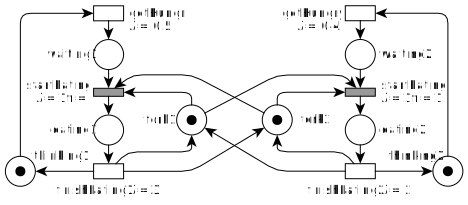
\includegraphics[scale=0.9]{figures/gspn_example}
  \caption{Example \textabbr{GSPN} for the dining philosophers problem.}
  \label{fig:background:gspn-example}
\end{figure}

\begin{runningExample}\label{ex:background:gspn}
  \Vref{fig:background:gspn-example} shows a \textabbr{GSPN} version of the dining philosophers model form \vref{ex:background:pn}. The timed transitions \lit{getHungry1}, \lit{getHungry2}, \lit{finishEating1} and \lit{finishEating2} have rates \(0.5\), \(0.45\), \(3.0\) and \(2.8\), respectively.

  The transitions \lit{startEating1} and \lit{startEating2} are immediate with equal priority and weight. Hence philosophers start eating as soon as they become hungry and there are forks available. Both philosophers can be selected to eat with equal priority if both are hungry at the same time.
\end{runningExample}

\subsubsection{Stochastic Petri nets}

A \emph{stochastic Petri net} (\textabbr{SPN}) is a \textabbr{GSPN} with no immediate transitions, i.e.~\(\pi(t) \equiv 0\) for all \(t \in T\). In such nets all reachable states are tangible, \(\textit{TRS} = \textit{RS}\).

Bounded \textAbbr{SPN}s can be transformed into \textAbbr{CTMC}s in a straightforward way. Let \(S = \{0, 1, \ldots, \lvert \textit{TRS} \rvert - 1\}\) be the set of states of the \textabbr{CTMC} and let \(\iota\colon \textit{TRS} \to S\) be a bijection. The off-diagonal elements of the infinitesimal generator matrix \(Q \in \RR^{\lvert \textit{TRS} \rvert \times \lvert \textit{TRS} \rvert}\) can be computed by summing the rates of transitions between states, while diagonal elements are set such that \(Q \vec{1}^T = \vec{0}^T\) is satisfied. Formally, we have
\begin{align}
  q[\iota(m), \iota(m')] &= \sum_{\mathclap{m \tranto{\scriptstyle t} m'}} \lambda(t) \quad\text{if \(m \ne m'\),}
  & q[x, x] &= - \sum_{y \ne x} q[x, y] \text.
\end{align}

This simple translation makes \textAbbr{SPN}s especially amenable to analysis. For \textAbbr{GSPNS} with immediate transitions the reachable vanishing markings must be \emph{eliminated} before a \textabbr{CTMC} can be formed~\citep{Marsan84gspn}.

\subsubsection{Marking- and parameter-dependent models}

The arc inscriptions of \textAbbr{GSPN}s can be made marking-dependent similarly to Petri nets, which lets the arcs \({\outarc}, {\inarc}, {\inharc} \subseteq P \times \Expr_P \times T\) contain arbitrary algebraic expressions of the token counts of the places \(P\). Moreover, the transition rates and weights can be made marking dependent, which results in \(\lambda\colon T \to \Expr_P\).

Dependence on a set of parameters \(\Par\) may also be introduced. In this case \(\lambda\colon T \to \Expr_{P, \Par}\), where \(\Expr_{P, \Par}\) is the set of algebraic expressions depending on token counts of \(P\) and the values of the parameters in \(\Par\). Parameter-dependent \textAbbr{GSPN}s are translated into parametric \textAbbr{CTMC}s, where the values of \(Par\) are encoded as the parameter vector \(\vec{\uptheta} \in A \subseteq \RR^{\lvert \Par \rvert}\). The feasible region \(A\) of parameter values can be determined according to domain requirements.

\subsubsection{Reward nets}

Generalized stochastic Petri nets can specify not only \textAbbr{CTMC}s, but also Markov reward models. The \emph{reward expression} \(r \in \Expr_P\) is an algebraic expression which may refer to token counts of places. The reward expression \(r\) is translated into a reward vector \(\vec{r}\) upon analysis in order to calculate expectations and answer queries regarding the reward value.

In the case of parameter-dependent \textAbbr{GSPN}s the reward expression may depend on the values of the parameters, such that we have \(r \in \Expr_{P, \Par}\).

\begin{runningExample}
  Consider the dining philosophers \textabbr{GSPN} from \vref{ex:background:gspn} along with the reward expression
  \begin{equation}
    r = \#\lit{thinking1} + \#\lit{thinking2} \text,
  \end{equation}
  which sums the token counts of the places \lit{thinking1} and \lit{thinking2}.

  The expected transient reward rate \(\Ex R(t)\) is the expected number of philosophers thinking at time \(t\) after starting from the initial marking. The expected steady-state reward rate \(\Ex R(\infty)\) is the mean number of thinking philosophers during long-term operation. The expected accumulated reward \(\Ex Y(t)\) is the mean total time spent thinking by philosophers until time \(t\) after starting.
\end{runningExample}

%%% Local Variables:
%%% mode: latex
%%% TeX-master: "../main"
%%% End:
